\section{Chemistry}

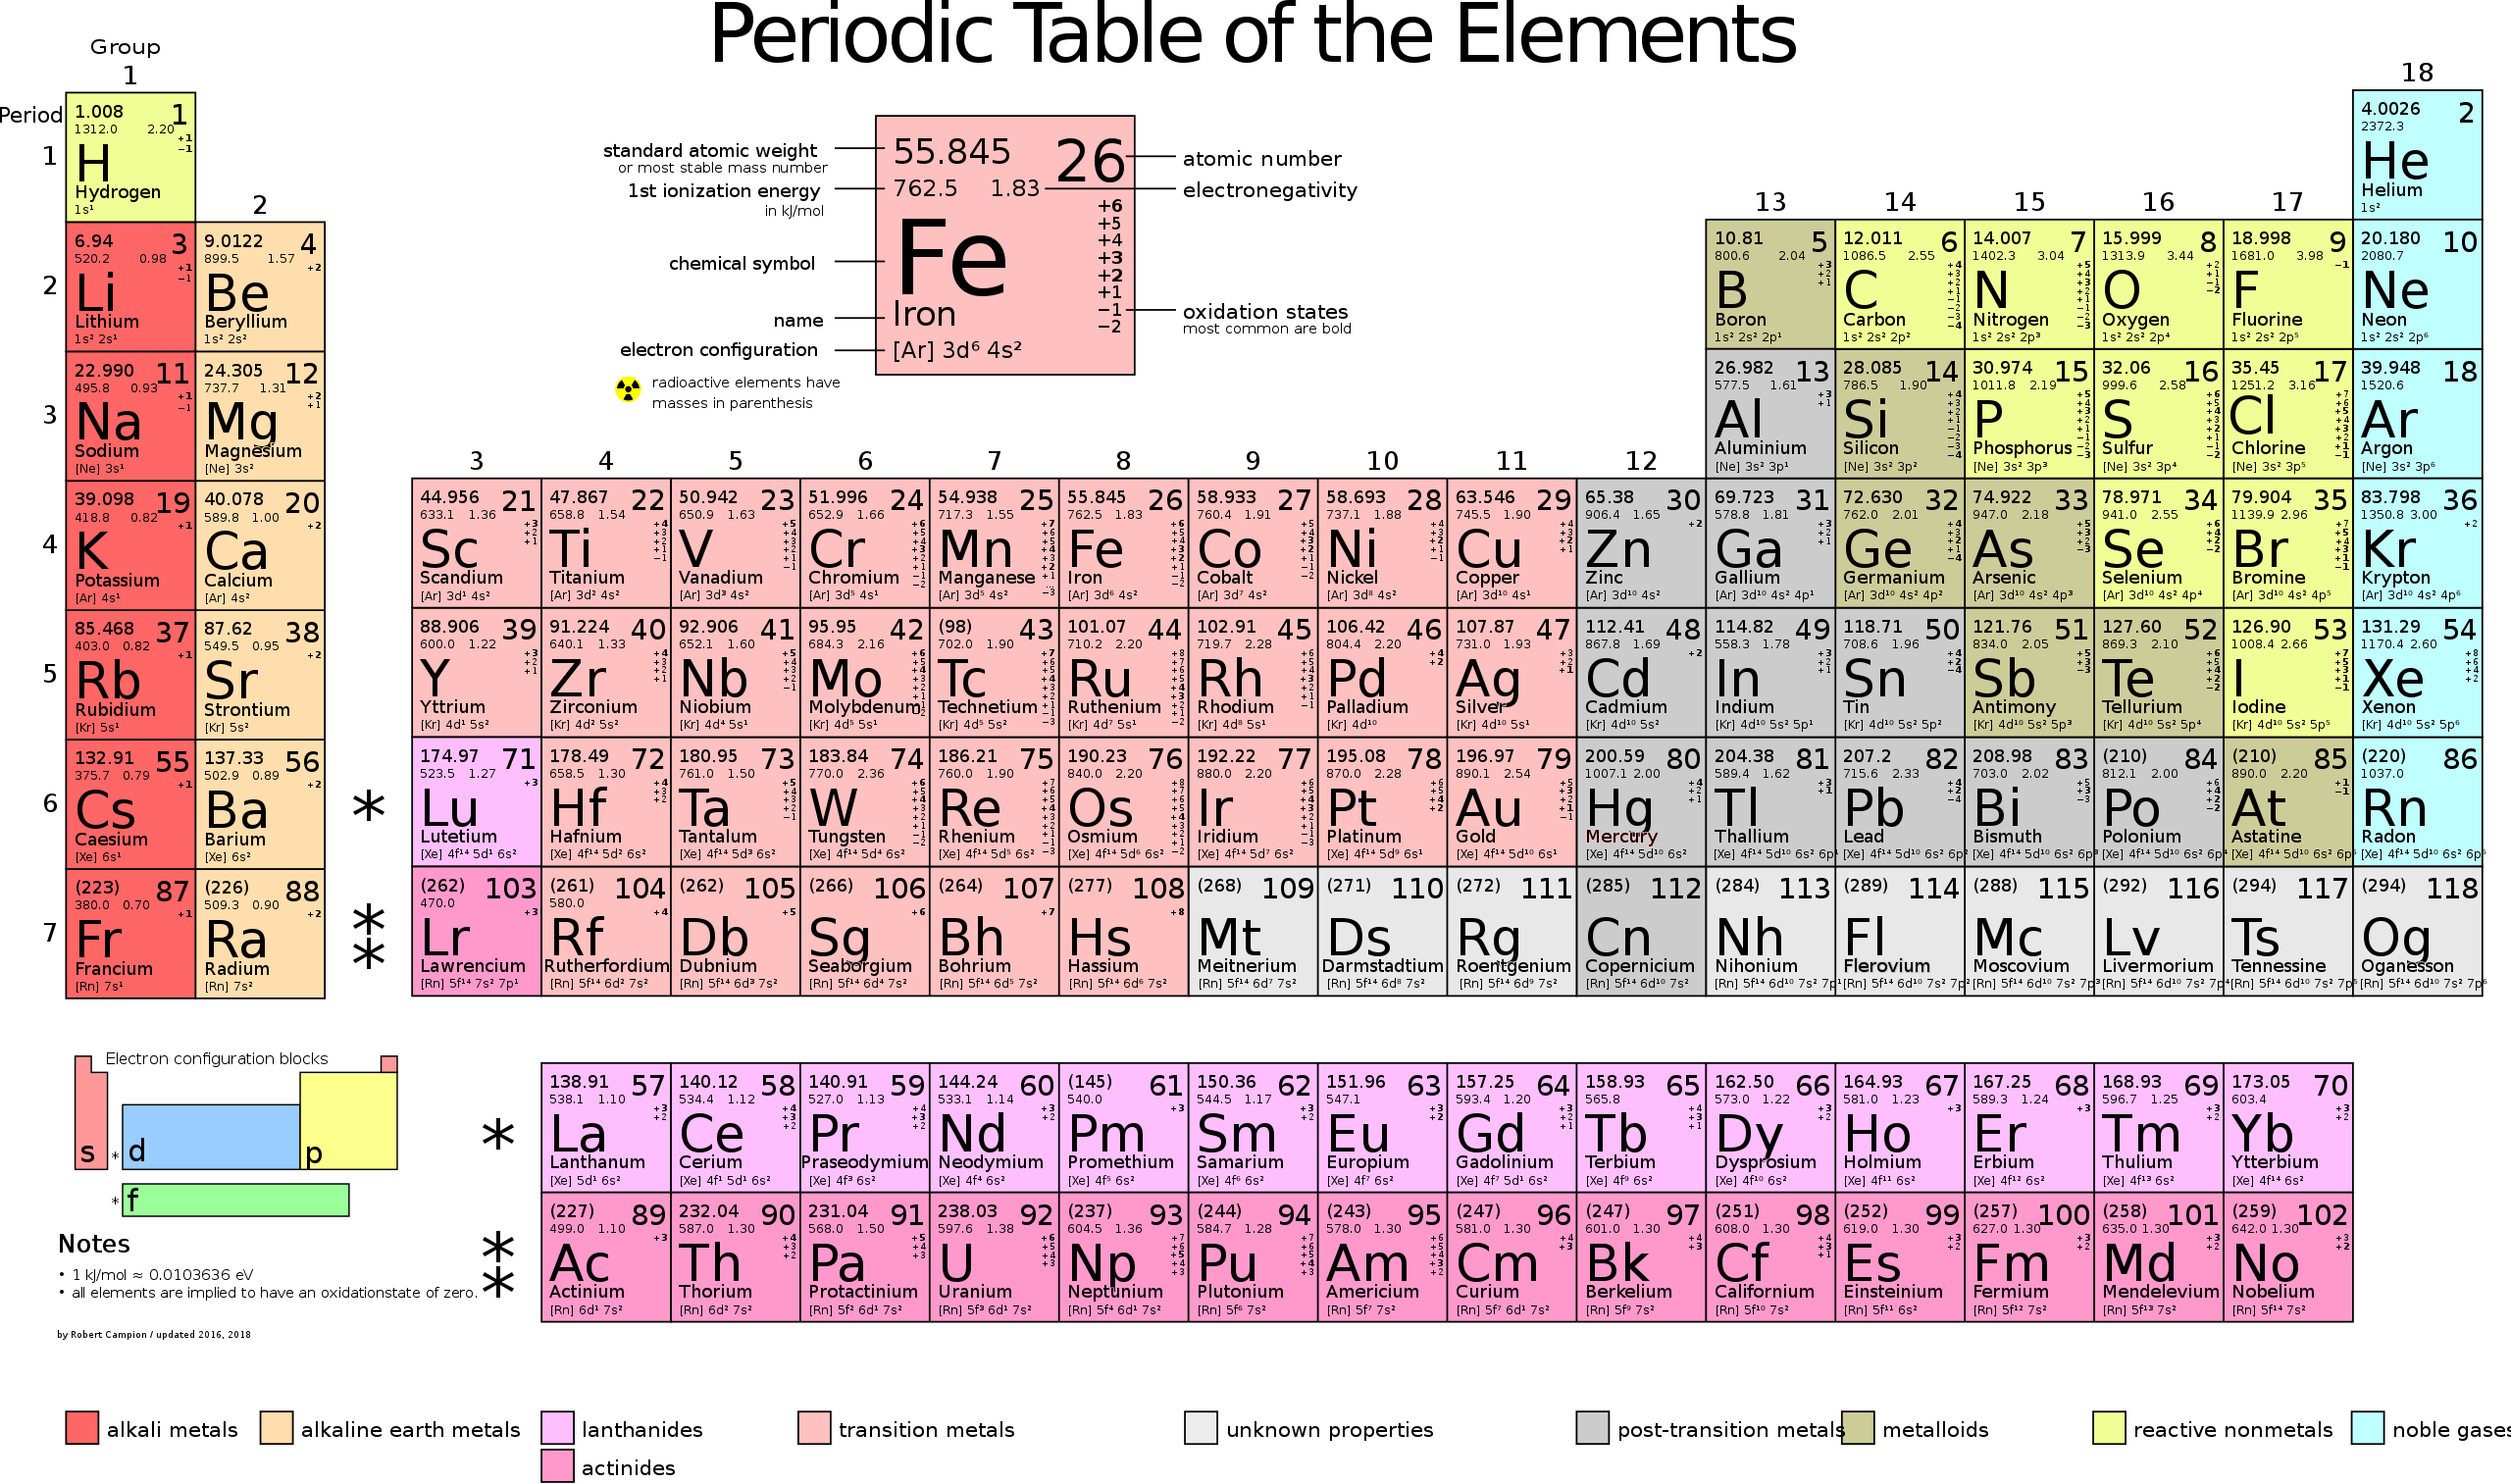
\includegraphics[width=\textwidth]{./chemistry/imgs/ptoe.png}
\href{https://www.youtube.com/watch?v=FSyAehMdpyI}{Crash Course Chemistry}

\subsection{Stoichiometry}
- amu = 1/12 the mass of an atom of $^{12}C$
- mol =  $6.022 x 10^{23}$
- Molarity = $M = \frac{\text{solute in moles}}{\text{solution\space in\space liters}}$
- Molality = $m = \frac{\text{solute in moles}}{\text{kg of solution}}$
- equation balancing => atom on lhs = atoms on rhs
- C~12~H~22~O~11~ + 12 O~2~ = 12 CO~2~ + 11 H~2~O

\subsection{Solution}
- solvent and solute
- aqueous solutions
- similar dissolve
-  H~2~O is polar => hydrophilic, lipophobic
-  is non-polar => lipophilic, hydrophobic
- Ions in solution are electrolytes => salts make water conductive

\subsection{Atoms}
- Brownian motion => random motion of particles suspended in a medium
- Neutron => atomic number
- Protons => stable / unstable
- Electron => negative

\subsection{Non metals}


\subsection{Non metals / metals}
- Salts
- Ions (Cations+,Anions-)
- Dissolved in water, they conduct electricity
- They are brittle [Spröd]

Par sa dilüi al ghe **gitterkräfte** ca ian da esa menu forti da **hydratasionsenergie**

\subsection{metals / metals}
- Atomic cores [Atomrümpfe]
- Electron gas => give away valence electrons easily

\subsection{Random}
- Water is at its densest at 4°C and ice floats on water
